%\documentclass[pdflatex,en,11pt]{aghdpl}
\documentclass[]{aghdpl}
\usepackage[polish]{babel}
\usepackage{polski}
\usepackage[utf8]{inputenc}
\usepackage{array}


\usepackage[backend=biber,
style=numeric,
%bibencoding=ascii,
%style=reading
giveninits=true
]{biblatex}
\renewbibmacro{in:}{%
    \ifentrytype{article}{}{\printtext{\bibstring{in}\intitlepunct}}}

\addbibresource{bibliografia.bib}

\DeclareNameAlias{sortname}{family-given}
\DeclareNameAlias{default}{family-given}

% dodatkowe pakiety
\usepackage{enumerate}
\usepackage{listings}
\usepackage{float}
\usepackage[binary-units=true]{siunitx}
\usepackage{hyperref}
\usepackage[acronym,nomain,toc]{glossaries}
\usepackage{multirow}
\usepackage{colortbl}
\usepackage{hhline}
\usepackage{lscape}
\usepackage{csquotes}

% \lstloadlanguages{TeX}

\lstset{
  literate={ą}{{\k{a}}}1
           {ć}{{\'c}}1
           {ę}{{\k{e}}}1
           {ó}{{\'o}}1
           {ń}{{\'n}}1
           {ł}{{\l{}}}1
           {ś}{{\'s}}1
           {ź}{{\'z}}1
           {ż}{{\.z}}1
           {Ą}{{\k{A}}}1
           {Ć}{{\'C}}1
           {Ę}{{\k{E}}}1
           {Ó}{{\'O}}1
           {Ń}{{\'N}}1
           {Ł}{{\L{}}}1
           {Ś}{{\'S}}1
           {Ź}{{\'Z}}1
           {Ż}{{\.Z}}1
}

\newcommand{\iic}{$I^2C$}
\newcommand{\uA}{\micro\ampere}
\newcommand{\mA}{\milli\ampere}
\newcommand{\uV}{\micro\volt}
\newcommand{\mV}{\milli\volt}
\newcommand{\Hz}{\hertz}
\newcommand{\kHz}{\kilo\hertz}
\newcommand{\MHz}{\mega\hertz}
\DeclareSIUnit{\belmilliwatt}{Bm}
\DeclareSIUnit{\belisotropic}{Bi}
\DeclareSIUnit{\dBm}{\deci\belmilliwatt}
\DeclareSIUnit{\dBi}{\deci\belisotropic}
\DeclareSIUnit{\ppm}{ppm}

\usepackage{array}
\newcolumntype{L}[1]{>{\raggedright\let\newline\\\arraybackslash\hspace{0pt}}m{#1}}
\newcolumntype{C}[1]{>{\centering\let\newline\\\arraybackslash\hspace{0pt}}m{#1}}
\newcolumntype{R}[1]{>{\raggedleft\let\newline\\\arraybackslash\hspace{0pt}}m{#1}}

\makeatletter
\let\ps@plain\ps@fancy
\makeatother

%---------------------------------------------------------------------------

\author{Filip Świątek}
\shortauthor{F. Świątek}

\course{Elektronika i Telekomunikacja}

\titlePL{Multiplekser interfejsu SWD}
\titleEN{SWD interface multiplexer}

\shorttitlePL{Multiplekser interfejsu SWD} % skrócona wersja tytułu jeśli jest bardzo długi
\shorttitleEN{SWD interface multiplexer}

\thesistypePL{Praca dyplomowa inżynierska}
\thesistypeEN{Bachelor Thesis}

\supervisorPL{dr inż. Łukasz Krzak}
\supervisorEN{Łukasz Krzak Ph.D}
\studytype{Stacjonarne}

\date{2019}

\departmentPL{Katedra Elektroniki}
\departmentEN{Department of Electronics}

\facultyPL{Wydział Informatyki, Elektroniki i Telekomunikacji}
\facultyEN{Faculty of Computer Science, Electronics and Telecommunications}

\acknowledgements{}

\setlength{\cftsecnumwidth}{10mm}
%---------------------------------------------------------------------------

\begin{document}

\titlepages
\tableofcontents
\clearpage
\chapter{Wstęp}
Celem pracy było zaprojektowanie i wykonanie multipleksera SWD (Serial Wire Debug) - urządzenia, które na podstawie komend przełącza linie sygnałowe interfejsu SWD pomiędzy programatorem a ośmioma urządzeniami docelowymi. Urządzenie powinno być sterowane i zasilane z USB, jednak dopuszcza się zasilanie jak i sterowanie poprzez interfejsy programatora.

\section{Potrzeba stworzenia urządzenia przełączającego}
Celem stworzenia multipleksera SWD było uproszczenie i automatyzacja procesu testowania oprogramowania dla urządzeń zbudowanych w oparciu o mikrokontroler. Ze względu na dużą popularność mikrokontrolerów wykorzystujących rdzenie z rodziny ARM Cortex-M, zdecydowano się na wykorzystanie interfejsu SWD (ang. Serial Wire Debug). Do jego zalet zaliczyć można szybkość programowania układów oraz małą liczbę wykorzystywanych wyprowadzeń. Wadą SWD względem popularnego w przeszłości standardu JTAG (ang. Joint Test Action Group) jest brak możliwości spięcia układów szeregowo w tzw. łańcuch (ang daisy chain), co pozwalało na programowanie wielu układów bez konieczności przepinania programatora. Brak tej funkcjonalności jest uciążliwy i Wiąże się z dużym problemem podczas programowania kilku urządzeń w krótkim odstępie czasu. \\
Programowanie wielu urządzeń na raz można zrealizować na 2 sposoby:
\begin{enumerate}
    \item Zastosowanie osobnego programatora dla każdego urządzenia docelowego. Wiąże się to ze znacznymi kosztami. Istnieje potrzeba zastosowania dużej ilości programatorów  (koszt jednego to nierzadko kilkaset a nawet kilka tysięcy PLN). Programatory te najczęściej są podłączane do komputera poprzez interfejs USB, a zatem w tym przypadku wymagane jest tyle samo portów USB co urządzeń docelowych. W przypadku indywidualnego projektu, małej lub nawet średniej firmy, koszty takiej automatyzacji stają się zbyt wysokie względem korzyści odniesionych w procesie tworzenia urządzeń docelowych.
    \item Przełączanie jednego programatora pomiędzy poszczególne urządzenia docelowe. Rozwiązanie znacznie tańsze, jednakże dla zwiększenia niezawodności poprzez ograniczenie wpływu zużycia gniazd i wtyczek, oraz ograniczenia wpływu błędu ludzkiego, należy zautomatyzować proces poprzez przełączanie linii sygnałowych pomiędzy urządzenia docelowe za pomocą dodatkowego urządzenia. Takim urządzeniem jest właśnie multiplekser SWD.
\end{enumerate}

Bezsprzecznie lepszym wyborem jest wybranie drugiej opcji ze względu na znacznie niższe koszty implementacji i znacznie mniej miejsca zajmowanego na stanowisku testowym. Wadami takiego rozwiązania jest czas poświęcony na opracowanie, wykonanie i testowanie urządzenia przełączającego, oraz fakt, że pomaga on jedynie w przypadku urządzeń wykorzystujących interfejs SWD.

\section{Prace wykonane w ramach projektu}
Prace w ramach projektu obejmowały:
\begin{enumerate}
    \item Weryfikację wstępną wykonalności projektu w rozsądnym czasie
    \item Wykonanie schematu blokowego urządzenia
    \item Dobór elementów ze względu na charakterystykę interfejsu SWD oraz możliwie jak najmniejszy rozmiar urządzenia
    \item Utworzenie schematu ideowego sprzętu
    \item Wykonanie projektu płytki drukowanej
    \item Napisanie oprogramowania układowego
    \item Stworzenie oprogramowania sterującego na PC
    \item Montaż elementów elektronicznych na płytce drukowanej
    \item Uruchomienie i sprawdzenie poprawności połączeń
    \item Końcowe testy oprogramowania i sprzętu
\end{enumerate}



\chapter {Interfejs SWD i programator}

Do komunikacji komputerów klasy PC poprzez interfejs SWD (Serial Wire Debug) używa się programatorów podpinanych do komputera przez port USB. Najpopularniejszy na rynku standard wyprowadzeń do obsługi urządzeń z rodziny ARM Cortex-M to ARM JTAG 20, posługujący się dwurzędowym wtykiem 2x10 pinów. Multiplekser SWD został stworzony do współpracy z takimi właśnie programatorami. Na potrzeby testów użyty został programator J-Link EDU. Jest to jeden z najpopularniejszych i tańszych programatorów, który posiada bardzo dobre wsparcie producenta, mogąc działać pod kontrolą systemów operacyjnych Windows, Linux i Mac OS.

\section{Serial Wire Debug}
 $SWD$, czyli Serial Wire Debug to standard interfejsu używany do komunikacji programatora z modułem $DAP$ (Debug Acces Protocol) w urządzeniach z rodziny ARM Cortex-M. Ponadro $SWD$ wymaga mniej wyprowadzeń niż konkurencyjny JTAG.\\
 Wykorzystuje on 2 linie transmisyjne:
 \begin{enumerate}
     \item $SWDIO$ - Dwukierunkowy sygnał danych.  
     \item $SWCLK$ - Sygnał zegara generowany przez sondę debugującą.
 \end{enumerate}
 Ponadto celem rozszerzenia funkcjonalności często używa się z nim linii:
 \begin{enumerate}
     \item $Reset$ -  sygnał reset, zwyczajowo aktywowany niskim stanem
     \item $SWO$ - Serial Wire Output - dedykowany do użycia jako asynchroniczne szeregowe standardowe wyjście. 
     \item $VTref$ - napięcie stanu wysokiego dla wyprowadzeń $SWD$
 \end{enumerate}
 
 \section{Programator J-Link EDU}
  Programator (inaczej sonda debugująca) J-Link EDU (rysunek \ref{J_Link_photo}) posiada interfejsy SWD, JTAG, SPI oraz UART. Wszystkie one mają bufory wejściowe i wyjściowe dopasowujące się do napięcia, jakim posługuje się urządzenie docelowe, przy czym napięcie dla stanu wysokiego musi się zawierać w przedziale od 1.2 V do 5 V a napięcie stanu niskiego to 0 V.
  Ponadto J-Link EDU od wersji V9 wspiera tzw. wirtualny port COM (VCOM), czyli port szeregowy UART w miejscu pinów 5 (Tx) oraz 17 (Rx). (schemat wyprowadzeń znajduje się na rysunku \ref{J_Link_SWD_pinout})
  Na pinie 5V-Supply można dodatkowo włączyć zasilanie 5 V, które może być użyte np. do zasilania urządzenia docelowego. Układ dodatkowo umożliwia pomiar prądu pobranego z tego wyprowadzenia.
  
\begin{figure}[H]
\centering
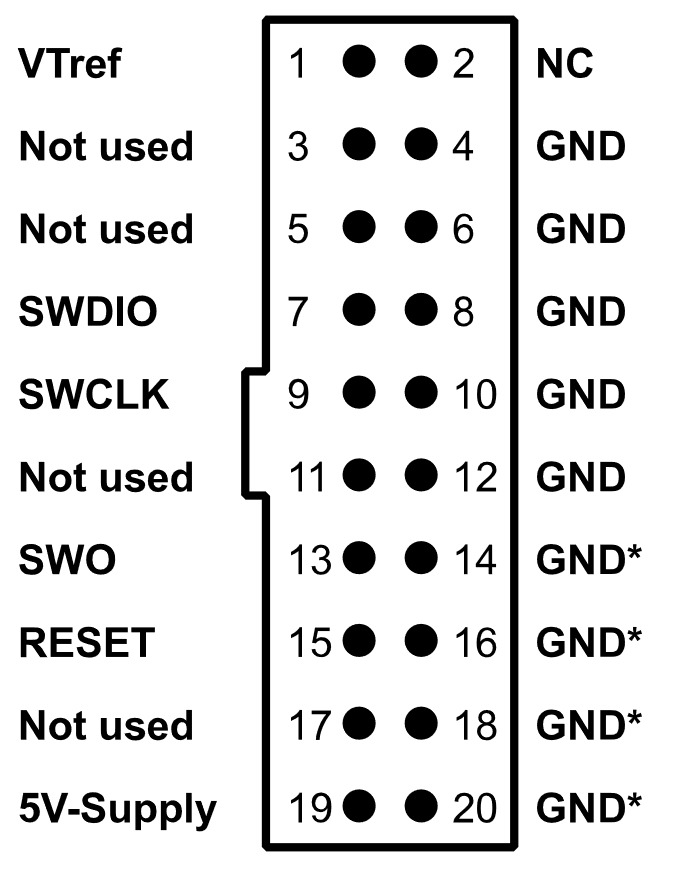
\includegraphics[width=0.35\paperwidth]{images/J-Link_pinout_SWD.png}
\caption{Schemat wyprowadzeń programatora J-Link EDU działającego w trybie SWD. Źródło:\cite{J-Link_pinout_SWD}}
\label{J_Link_SWD_pinout}
\end{figure}

   \begin{figure}[H]
    \centering
    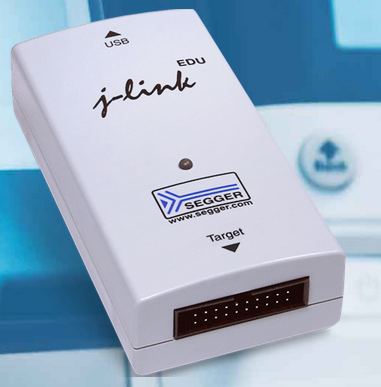
\includegraphics[width=0.45\paperwidth]{images/J-Link_EDU.png}
    \caption{Programator J-Link EDU Źródło:\cite{J-Link_EDU_photo}}
    \label{J_Link_photo}
\end{figure}

  


 



\chapter{Komunikacja programatora i komputera z multiplekserem SWD}
Multiplekser SWD nie jest urządzeniem w pełni samodzielnym. Potrafi co prawda przełączać urządzenia docelowe reagując na wciśnięcie przycisku, lecz jego integralną cechą jest reakcja na dane wysyłane przez komputer.

\section{Połączenie SWD między programatorem a multiplekserem SWD}
Między programatorem a multiplekserem SWD należy poprowadzić 20-żyłową taśmę AWG28 zakończoną z dwóch stron wtyczką IDC20 o rozstawie wyprowadzeń 2.45mm. Należy ograniczać jak najbardziej długość połączenia ze względu na wpływ indukcyjności i pojemności pasożytniczych przewodów, oraz na fakt, że im krótsze połączenie, tym mniejszy wpływ zjawisk tzw. linii długiej.

\section {Sterowanie multiplekserem SWD}
Jednym z założeń projektu była ścisła kontrola urządzenia po stronie komputera, dlatego multiplekser SWD nasłuchuje instrukcji poprzez wiersz poleceń, zgłaszając się w systemie jako port komunikacyjny (serial port). Po stronie multipleksera SWD zaimplementowano interfejs USB-CDC (USB communications device class). Dzięki temu urządzenie nie wymaga instalacji dodatkowego sterownika. Wadą takiego rozwiązania jest wybranie numeru konkretnego urządzenia (multipleksera SWD) w systemie operacyjnym.
Komendy występują w następującej składni: \newline
[nazwa komendy] [znak odstępu ($0x20$ w ASCII)] [argument] [znak nowej linii ($0x0A$ w ASCII)]\\
Dostępne są dwie komendy:
\begin{enumerate}
    \item select [numer urządzenia docelowego] \\
    Komenda ta przełącza urządzenie docelowe.
    Argumentem polecenia jest numer tego urządzenia (z przedziału 0-7) 
    \item reset\_all [set/clear/[brak opcji]] \\
    Komenda resetuje jednocześnie wszystkie urządzenia docelowe.
    Argumenty to kolejno:
    \begin{enumerate}
        \item set - Zwiera linię reset do masy, odłączywszy wcześniej sygnał z J-Linka dla tej linii. 
        \item clear - Przełącza źródło sygnału reset z powrotem na J-Linka
        \item [brak opcji] - Skutkuje impulsem resetującym trwającym 40 ms. (skutek taki sam jak uruchomienie komendy z argumentem set a następnie clear po 40 ms).
    \end{enumerate}
\end{enumerate}

W przypadku powodzenia podczas wykonania komendy, urządzenie wysyła komunikat \enquote{OK}. W przeciwnym razie komunikat zwrotny to \enquote{ERR}.
\chapter{Część sprzętowa} 

\section {Schemat blokowy multipleksera SWD oraz jego użycia}

Rysunek \ref{SWD_multiplexer block diagram} przedstawia schemat blokowy multipleksera. Składa się on z poniższych bloków:
\begin{enumerate}
    \item STM32F103C8 MCU - mikrokontroler odpowiedzialny za sterowanie pozostałymi częściami multipleksera SWD i komunikację z komputerem
    \item szereg diod - wskaźniki obecnie wybranego urządzenia docelowego
    \item wtyczka 20 pin w standardzie ARM JTAG
    \item szereg multiplekserów analogowych 1 do 8 - szczegółowy schemat na rysunku \ref{mux_matrix diagram}
    \item 16 wtyczek do urządzeń docelowych (z powodu zastosowania zarówno standardu pochodzącego z zespołu Bezprzewodowych Sieci Kontrolno-Pomiarowych Katedry Elektroniki AGH (WSN AGH)  jak i CoreSight złącz jest 2 razy więcej niż minimalna wymagana ilość)
\end{enumerate}

 \begin{figure}[H]
    \centering
    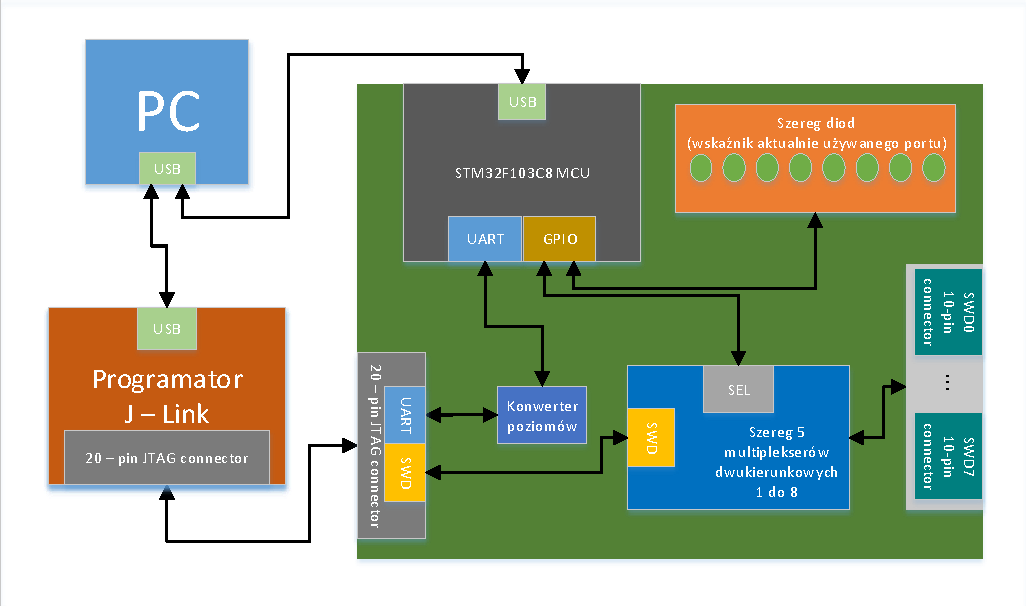
\includegraphics[width=0.75\paperwidth]{images/blokowy_hardware_main.pdf}
    \caption{{Schemat blokowy multipleksera SWD oraz sposób podpięcia urządzeń nadrzędnych.}}
    \label{SWD_multiplexer block diagram}
\end{figure}

 \begin{figure}[H]
    \centering
    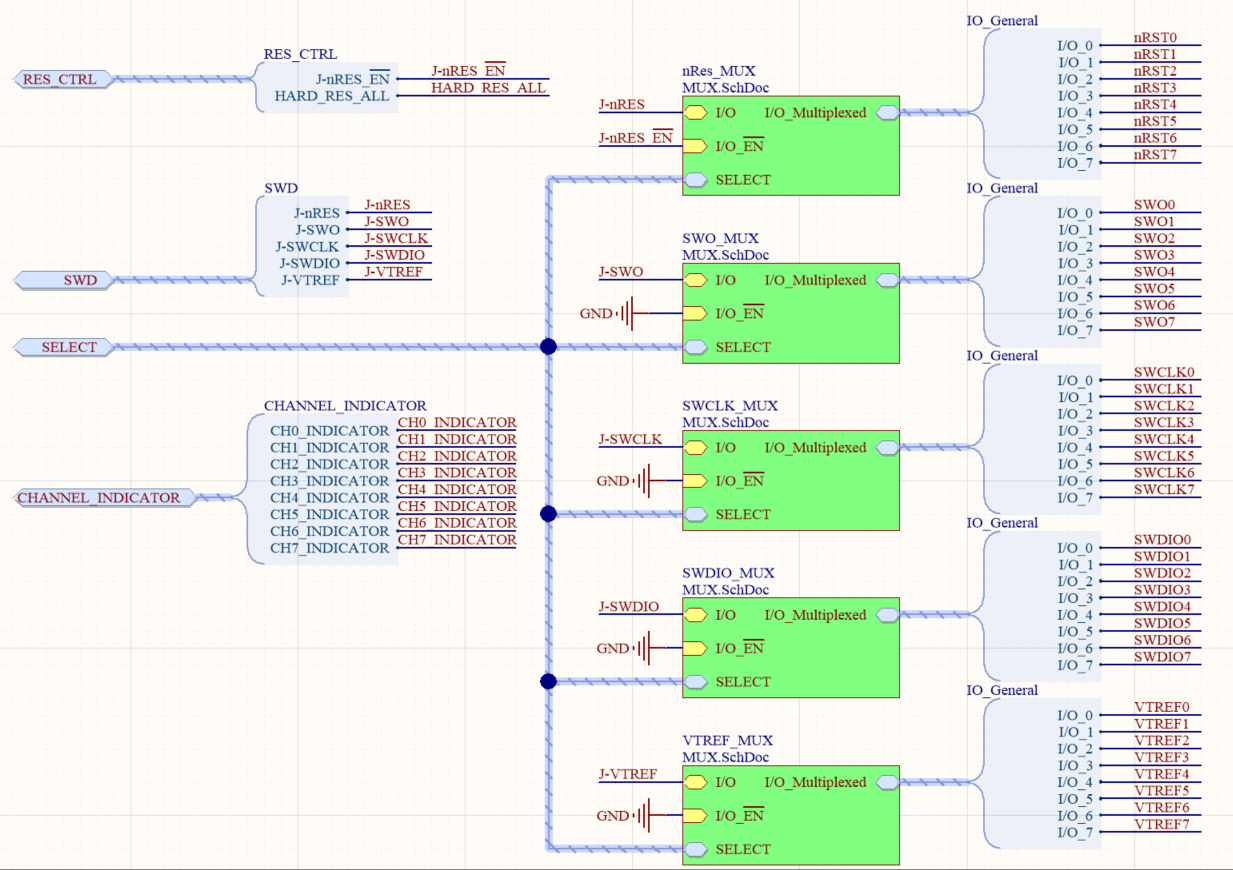
\includegraphics[width=0.8\paperwidth]{images/mux_matrix.png}
    \caption{{Schemat szczegółowy szeregu 5 multiplekserów dwukierunkowych.}}
    \label{mux_matrix diagram}
\end{figure}

Na rysunku \ref{mux_matrix diagram} znajduje się szczegółowy schemat wewnętrzny bloku \enquote{Szereg 5 
multiplekserów 
dwukierunkowych 1 do 8} z rysunku  \ref{SWD_multiplexer block diagram}.
Pokazuje on sposób połączenia multiplekserów analogowych przełączających linie sygnałowe interfejsu SWD. Bloki o nazwie zakończonej na \enquote{MUX} posiadają wewnętrzny schemat na rysunku \ref{SN74CBT3251_connection}.
Magistrala \enquote{RES\_CTRL} steruje włączeniem multipleksera \enquote{nRes\_MUX}, co z kolei pozwala na opięcie sygnału reset z programatora i sterowanie nim w każdym urządzeniu docelowym poprzez tranzystor zwierający ten sygnał do masy (Tranzystor ten poziada oznaczenie Q1 na ryzunku \ref{target_connectors}).


\section{Sekcja zasilania}
Układ zasilany jest z portu USB lub z programatora. Wymaga to użycia diod (D9 i D10 na schemacie), które zabezpieczałyby przed zwarciem w przypadku podłączenia na raz obu źródeł zasilania. Zasilacz podaje kolejno napięcia:
\begin{enumerate}
    \item 5 V, niestabilizowane\\
    Linia 5 V używana jest do zasilania multiplekserów analogowych, oraz stabilizatorów liniowych dla linii 3.3 V oraz 1.8 V. Schemat na rysunku \ref{5V_power_supply}
    \begin{figure}[H]
    \centering
    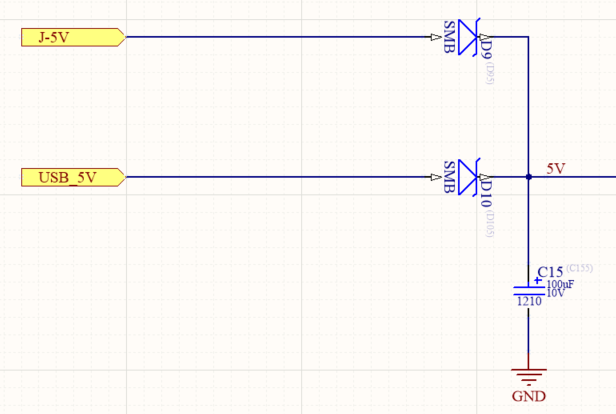
\includegraphics[width=0.35\paperwidth]{images/5V_supply.png}
    \caption{sekcja 5 V zasilacza}
    \label{5V_power_supply}
    \end{figure}

    \item 3.3 V, stabilizowane \\
    Linia ta jest używana do zasilania mikrokontrolera STM32F103C8, oraz służy jako jedno z napięć odniesienia dla konwertera stanów logicznych. Z tego źródła zasilana jest dioda "Power" wskazująca włączenie urządzenia.
    Schemat na rysunku \ref{3.3V_power_supply}
    
    \begin{figure}[H]
    \centering
    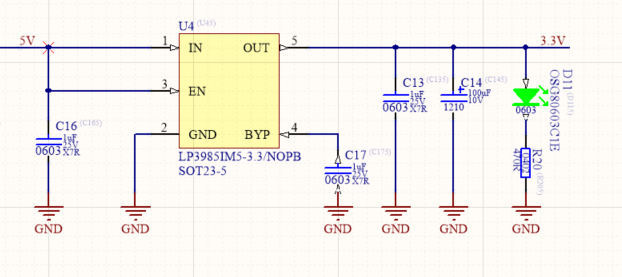
\includegraphics[width=0.55\paperwidth]{images/3,3V_supply.png}
    \caption{sekcja 3.3 V zasilacza}
    \label{3.3V_power_supply}
    \end{figure}
    
    \item 1.8 V, stabilizowane\\
    To źródło zasilania służy jedynie jako źródło napięcia 1.8V dla jednego z konwerterów stanów logicznych.  
    Schemat na rysunku \ref{1.8V_power_supply}
    
    \begin{figure}[H]
    \centering
    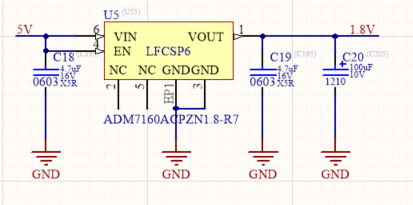
\includegraphics[width=0.45\paperwidth]{images/1,8V_supply.png}
    \caption{sekcja 1.8 V zasilacza}
    \label{1.8V_power_supply}
    \end{figure}
    
\end{enumerate}

\section{Realizacja sprzętowa interfejsów komunikacyjnych USB i UART}

Programator J-Link, który może zostać użyty jako urządzenie sterujące poprzez interfejs UART, dostosowuje poziomy wejściowe i wyjściowe interfejsów do napięcia referencyjnego (napięcie zasilania urządzenia docelowego.) Z racji faktu iż multiplekser SWD zaprojektowany jest pod kątem urządzeń pracujących z napięciami zasilania od 1.8V do 5V, J-Link nie będzie pracował jedynie na napięciu 3.3 V (jest to napięcie zasilania mikrokontrolera osadzonego na płycie multipleksera SWD). Tworzy to potrzebę konwersji poziomów dla samego interfejsu UART. Wygodny do takich zastosowań jest układ TXS0102YZPR, konwertujący poziomy logiczne. Układ ten ma jednak ograniczenie polegające na tym, że jedno z wejść musi mieć zagwarantowany wyższy bądź równy poziom napięcia odniesienia. W tym projekcie tak by nie było, gdyż, urządzenia docelowe mają pracować pomiędzy 1.8 V a 5V. Rozwiązaniem problemu było dodanie dodatkowego stopnia przejściowego na napięciu 1.8 V. Dlatego właśnie w projekcie użyto dwóch układów TXS0102YZPR.
Ogólne i szczegółowe schematy połączeń konwerterów poziomów znajdują się na rysunkach \ref{UART_level_shifters} oraz \ref{level shifter component sheet}

\begin{figure}[H]
    \centering
    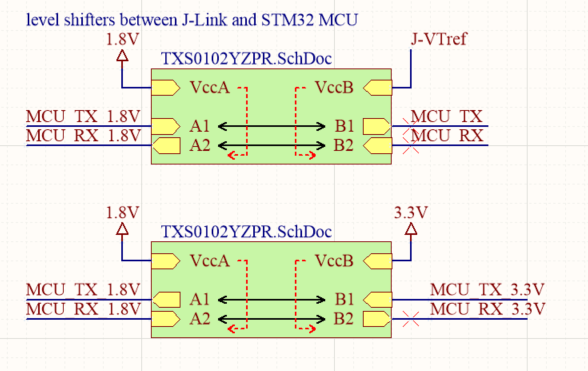
\includegraphics[width=0.55\paperwidth]{images/MCU_level_shifters.png}
    \caption{schemat blokowy układu konwerterów poziomów logicznych}
    \label{UART_level_shifters}
\end{figure}

\begin{figure}[H]
    \centering
    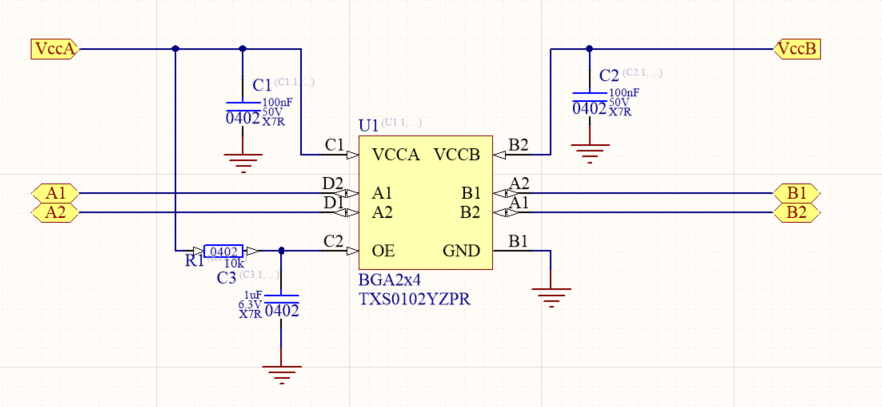
\includegraphics[width=0.55\paperwidth]{images/level_shifter_component_sheet.png}
    \caption{schemat podłączenia  układu $TXS0102YZPR$}
    \label{level shifter component sheet}
    \end{figure}

\section{Problem różnych napięć zasilania urządzeń docelowych}
Możliwość działania do 8 urządzeń docelowych pracujących w różnych standardach napięcia dla stanu wysokiego wymaga użycia sygnału zwrotnego napięcia referencyjnego (celem przekazania go do programatora). W takim wypadku niezbędne jest użycie analogowego multipleksera, gdyż przenosi on sygnał na zasadzie połączenia, nie zmieniając przy tym wartości napięcia. Sygnał SWDIO jest ponadto sygnałem dwukierunkowym, dlatego najłatwiejszym sposobem jego przełączania jest użycie multipleksera analogowego. Nic nie stoi na przeszkodzie użycia takich samych multiplekserów na pozostałych liniach sygnałowych.

\section{Multipleksacja sygnałów}
Przełączanie sygnałów zostało zrealizowane poprzez pięć multiplekserów analogowych $SN74CBT3251$ firmy Texas Instruments. Układ ten został wybrany ze względu na odpowiednio niskie czasy propagacji sygnału. (tabela \ref{tab:mux_propagation_table}) Wymaganie to jest konieczne, aby spełnić zapotrzebowanie na szybkozmienne sygnały celem przyspieszenia debugowania lub wgrywania oprogramowania do pamięci mikrokontrolera docelowego. Ma to znaczenie zwłaszcza w przypadku aż ośmiu urządzeń docelowych. Zasilanie takiego układu nie jest bardzo wymagające - zmiany tego napięcia wpływają jedynie na szybkość propagacji.

\begin {table}[H]
\begin{center}
\begin{tabular}{ |c|c|c|c|c|c| } 
\hline
parametr & Z (wejście) & Do (wyjście) & Vcc &  max & jednostka\\
\hline
\multirow{1}{*}[-7.5pt]{czas propagacji} & \multirow{1}{*}[-7.5pt]{A lub B} & \multirow{1}{*}[-7.5pt]{B lub A} & $Vcc = 4 V$          & $0.35$ & ns\\
&                       &      & $Vcc = 5 V \pm 0.5 V$  & $0.24$ & ns\\ 
\hline
\multirow{1}{*}[-7.5pt]{czas propagacji} & \multirow{1}{*}[-7.5pt]{S} & \multirow{1}{*}[-7.5pt]{A} & $Vcc = 4 V$          & $6$ & ns\\
&                       &      & $Vcc = 5 V \pm 0.5 V$  & $5.5$ & ns\\ 
\hline
\multirow{1}{*}[-7.5pt]{czas aktywacji} & \multirow{1}{*}[-7.5pt]{S} & \multirow{1}{*}[-7.5pt]{B} & $Vcc = 4 V$          & $6.4$ & ns\\
&                       &      & $Vcc = 5 V \pm 0.5 V$  & $5.8$ & ns\\ 
\hline
\end{tabular}
\caption{Parametry propagacyjne multipleksera analogowego $SN74CBT3251$ . Źródło:\cite{SN74CBT3251_datasheet_propagation}}
\label{tab:mux_propagation_table}
\end{center}
\end {table}

\begin{figure}[H]
    \centering
    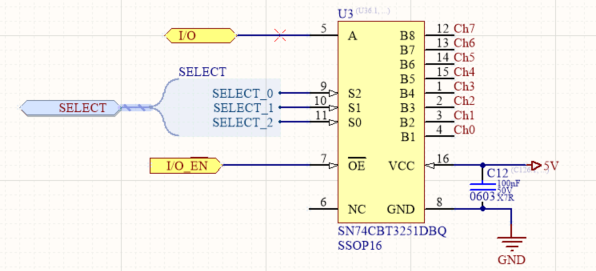
\includegraphics[width=0.6\paperwidth]{images/MUX_connection.png}
    \caption{Schemat połączenia multipleksera analogowego $SN74CBT3251$.}
    \label{SN74CBT3251_connection}
\end{figure}

Na schemacie można zobaczyć błąd powstały podczas projektowania obwodu sterowania multiplekserem. Sygnały SELECT\_0 i SELECT\_2 zostały omyłkowo podłączone na odwrót. Problem ten jednak został wykryty i poprawiony na etapie testów. Błędne działanie zostało skorygowane poprzez podmianę zachowań wyprowadzeń GPIO w oprogramowaniu.


\section{Zabezpieczenia przeciwprzepięciowe i przeciwzakłóceniowe}
Każde z wyjść multiplekserów zabezpieczone jest dolnoprzepustowymi filtrami przeciwzakłóceniowymi i przeciwprzepięciowymi. Ma to na celu uniknięcie uszkodzenia multipleksera z w przypadku wystąpienia krótkotrwałego potencjału wyższego niż 5V pochodzącego od strony urządzeń docelowych (np. dotknięcie wyprowadzeń dłonią naładowanego elektrycznie użytkownika - ESD). Filtrację tę wykonają układy scalone $EMI5208MUTAG$. Każdy z nich filtruje po 8 linii sygnałowych.

 \begin{figure}[H]
    \centering
    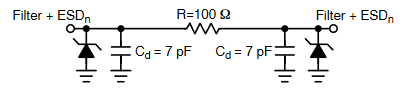
\includegraphics[width=0.7\paperwidth]{images/EMI5208MUTAG_internal_schematic.png}
    \caption{Schemat wewnętrzny filtra $EMI5208MUTAG$ . Źródło:\cite{EMI5208MUTAG_datasheet}}
    \label{EMI5208MUTAG_internal_schematic}
\end{figure}

 \begin{figure}[H]
    \centering
    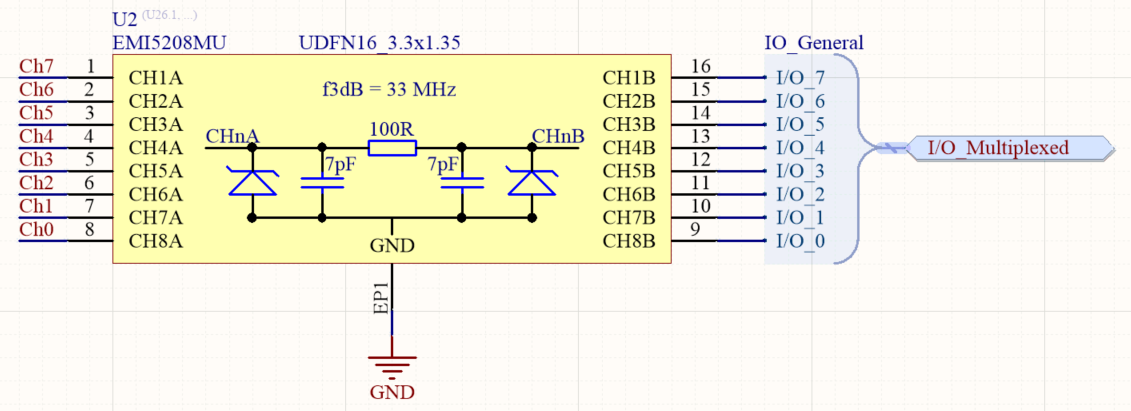
\includegraphics[width=0.7\paperwidth]{images/EMI_connection.png}
    \caption{Schemat połączenia filtra $EMI5208MUTAG$ .}
    \label{EMI5208MUTAG_connection diagram}
\end{figure}


Zabezpieczony został także port mini USB. Dla osiągnięcia bezproblemowego połączenia, użyty został dedykowany temu zastosowaniu układ scalony: USBLC6-2SC6. Układ ten oparty jest na pięciu diodach transil, które gwarantują zabezpieczenie zarówno linii zasilającej jak i dwóch linii danych zapewniając przy tym transmisję USB 2.0 high speed (480Mb/s).
Jednocześnie układ zapewnia niski pobór pasożytniczego prądu (do 150 nA) oraz niewielką pojemność pasożytniczą (maksymalnie 3.5 pF).

\begin{figure}[H]
    \centering
    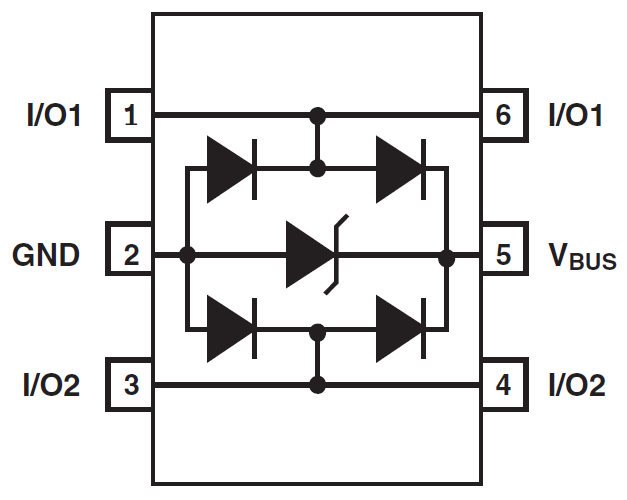
\includegraphics[width=0.45\paperwidth]{images/USBLC6-2SC6_internal_schematic.png}
    \caption{Schemat wewnętrzny filtra $USBLC6-2$ . Źródło:\cite{USBLC6-2_datasheet}}
    \label{USBLC6-2SC6_internal_schematic}
\end{figure}


\begin{figure}[H]
    \centering
    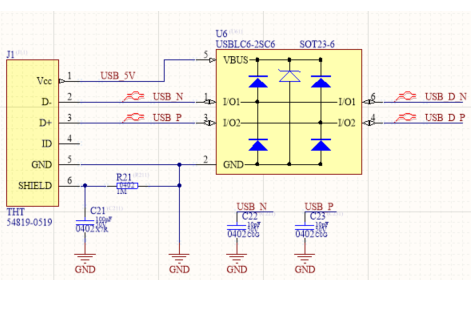
\includegraphics[width=0.8\paperwidth]{images/USB_ESD_protection2.png}
    \caption{Schemat połączenia filtra $USBLC6-2$ i gniazda mini USB.}
    \label{USBLC6-2SC6_connection}
\end{figure}

\section {Przyciski}
Przyciski to przełączniki typu tactswitch. (rysunek \ref{tactswitches}) Celem uproszczenia oprogramowania zdecydowano o eliminacji wpływu zjawiska drgania styków sposobem sprzętowym poprzez zastosowanie kondensatorów gaszących oscylacje.

\begin{figure}[H]
    \centering
    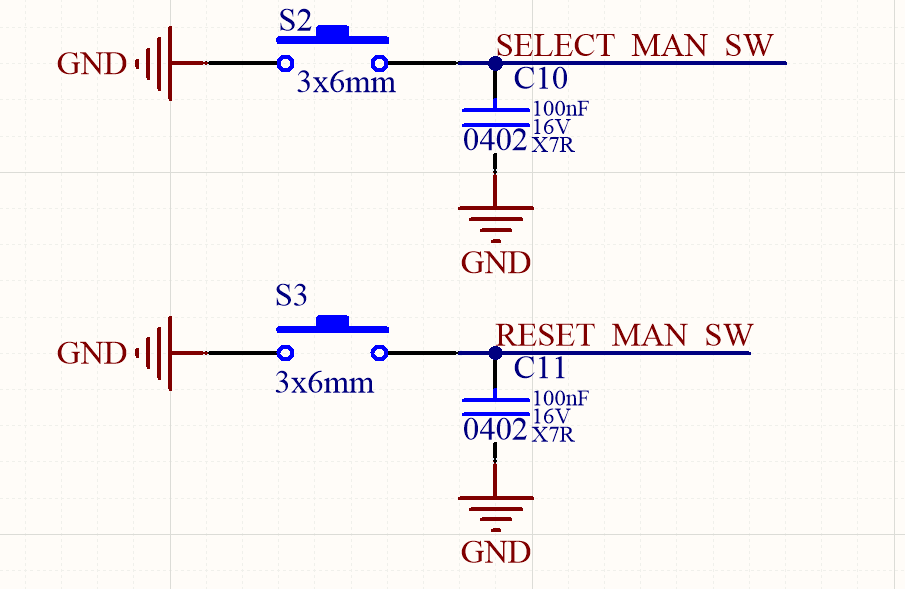
\includegraphics[width=0.7\paperwidth]{images/MCU_switches_debouncing.png}
    \caption{Schemat połączenia przycisków.}
    \label{tactswitches}
\end{figure}


\section{Gniazda zastosowane do podłączenia urządzeń docelowych}

Do podpięcia urządzeń docelowych użyto dwóch rodzajów gniazd. Wynika to z wymaganej zgodności z urządzeniami docelowymi zaprojektowanymi dotychczas w zespole Bezprzewodowych Sieci Kontrolno-Pomiarowych Katedry Elektroniki AGH (złącza bez plastikowej otoczki, rysunek \ref{WSN_Connector}) oraz pełnej kompatybilności z urządzeniami docelowymi wykorzystującymi standard CoreSight 10. Dodatkowo rozszerzono funkcjonalność gniazd zgodnych ze standardem CoreSight10 o wyprowadzenia portu szeregowego UART w miejscu klucza, który nie jest podpięty do żadnego sygnału, oraz w miejsce pinu nieużywanego w trybie SWD. (rysunek \ref{CoreSight10_capable_Connector}) W trybie zgodności z J-TAG pin ten służył jako sygnał TDI. 
Złącza interfejsu UART z gniazd prowadzących do urządzeń docelowych zostały wyprowadzone na złączach szpilkowych o rozstawie 2.54 mm. (złącze oznaczone jako P4 na rysunku \ref{target_connectors}) Ma to na celu możliwość podpięcia zewnętrznego monitora portu szeregowego.


\begin{figure}[H]
  \centering
  \begin{minipage}[b]{0.4\textwidth}
    \centering
    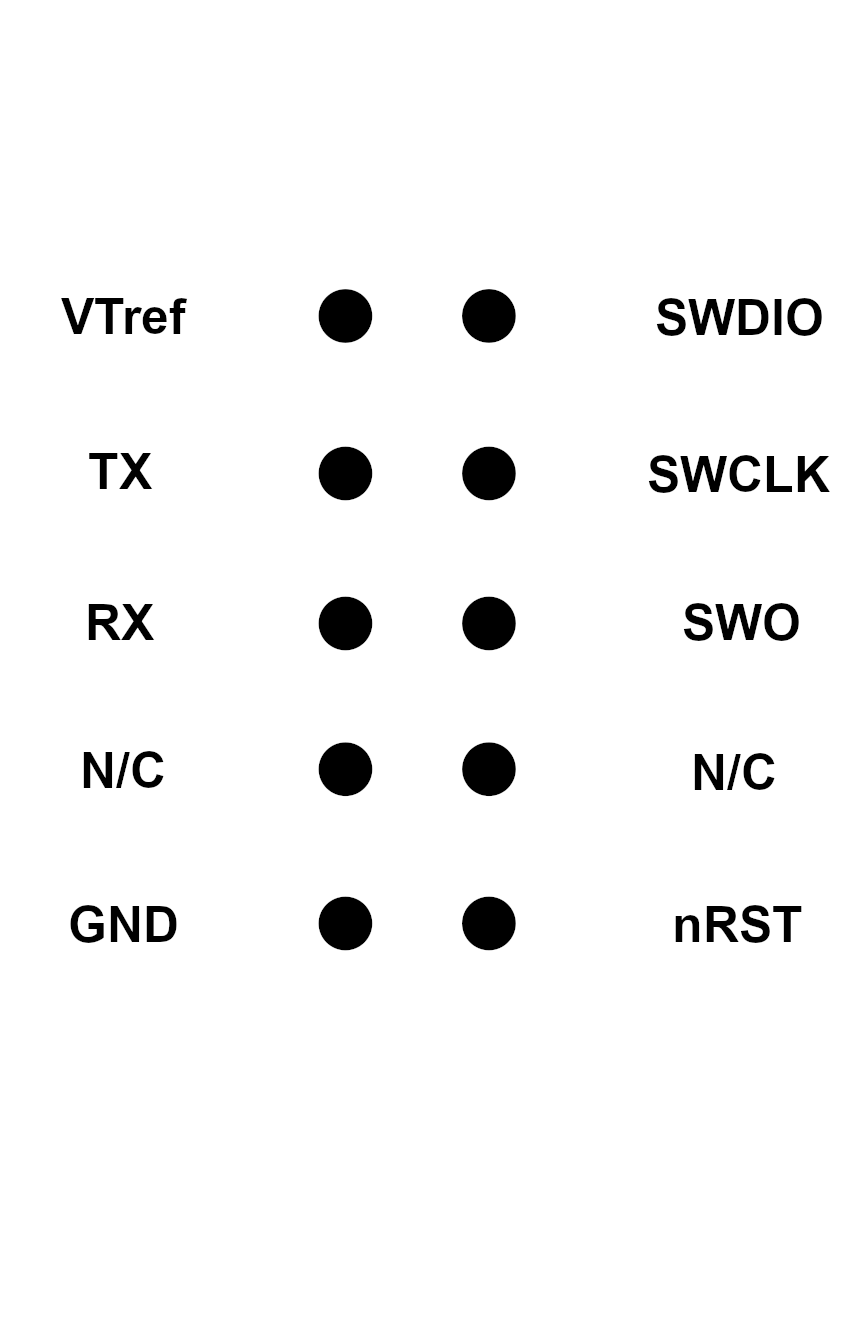
\includegraphics[height=0.4\paperwidth]{images/WSN_plug.png}
    \caption{Schemat wyprowadzeń wtyczki opracowanej w WSN AGH.}
    \label{WSN_Connector}
  \end{minipage}
  \hfill
  \begin{minipage}[b]{0.4\textwidth}
    \centering
    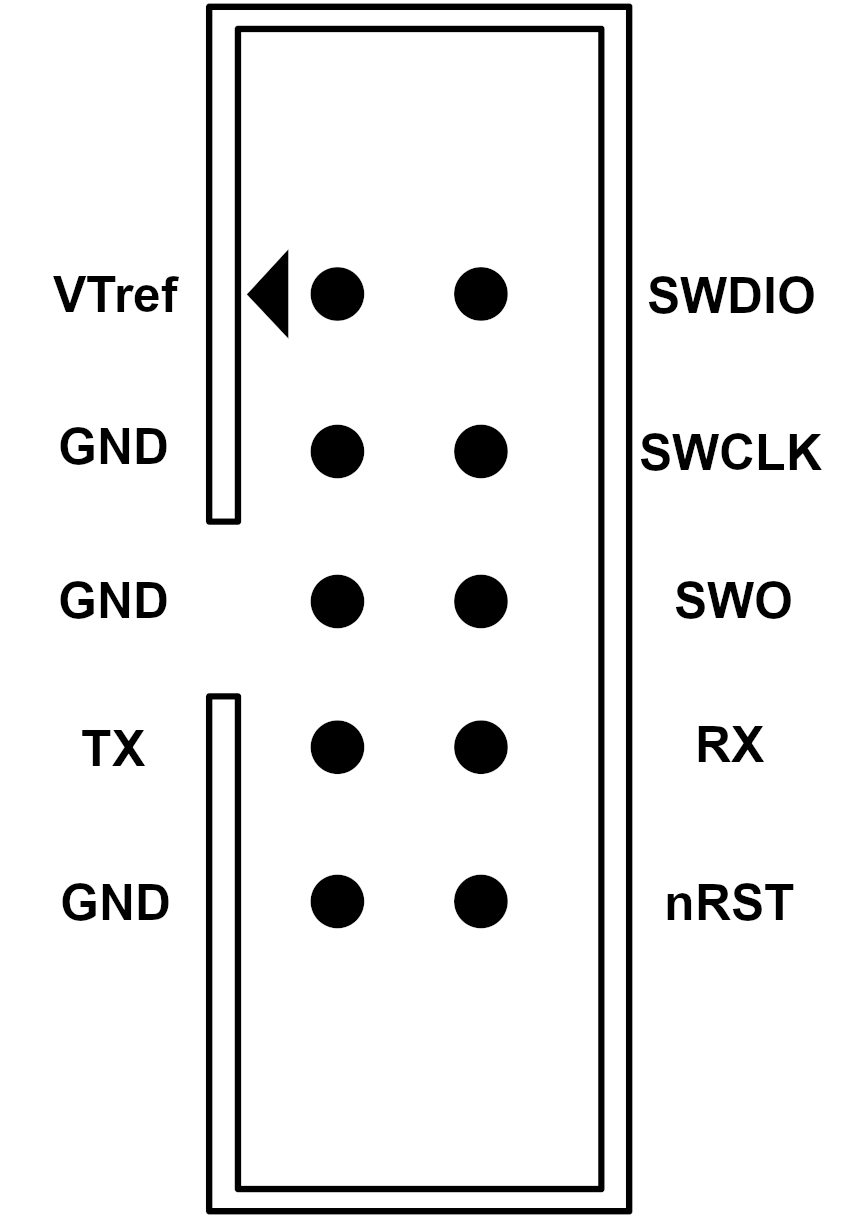
\includegraphics[height=0.4\paperwidth]{images/CoreSight10.png}
    \caption{Schemat wyprowadzeń wtyczki zgodnej z CoreSight10. Źródło:\cite{CoreSight10_documentation} }
    \label{CoreSight10_capable_Connector}
  \end{minipage}
\end{figure}

\begin{figure}[H]
    \centering
    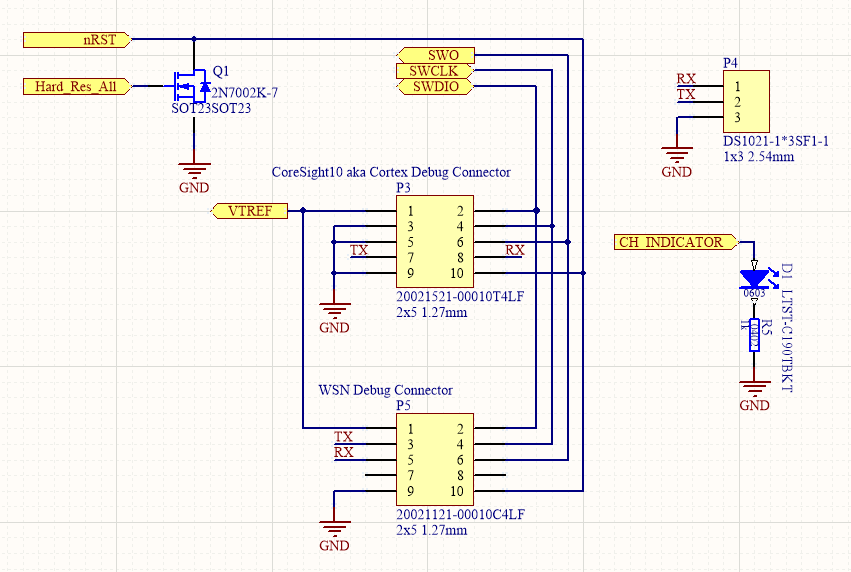
\includegraphics[width=0.75\paperwidth]{images/target_connectors.png}
    \caption{Schemat połączenia wyprowadzeń gniazd w stronę urządzenia docelowego.}
    \label{target_connectors}
\end{figure}



\section{Połączenie wyprowadzeń mikrokontrolera}

W projekcie użyto  mikrokontrolera STM32F103C8. To popularny mikrokontroler posiadający między innymi interfejs USB, który nie wymaga dodatkowego układu scalonego odpowiedzialnego za konwersję interfejsów. Pomaga to zaoszczędzić miejsce na płycie PCB oraz zminimalizować koszty produkcji urządzenia. Mikrokontroler zawiera wbudowaną pętlę PLL, która pozwala uzyskać częstotliwość taktowania zegara procesora do 72MHz przy rezonatorze wykorzystującym kryształ kwarcowy o częstotliwości oscylacji 16MHz.

\begin{figure}[H]
    \centering
    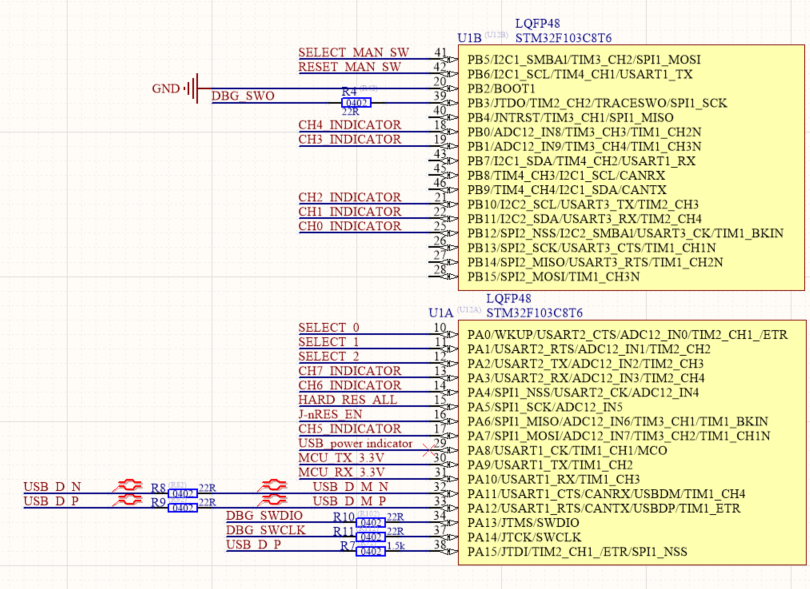
\includegraphics[width=0.65\paperwidth]{images/MCU_STM32.png}
    \caption{Schemat połączenia wyprowadzeń mikrokontrolera STM32F103C8 odpowiedzialnych za urządzenia wejścia-wyjścia}
    \label{MCU_STM32}
\end{figure}

\begin{figure}[H]
    \centering
    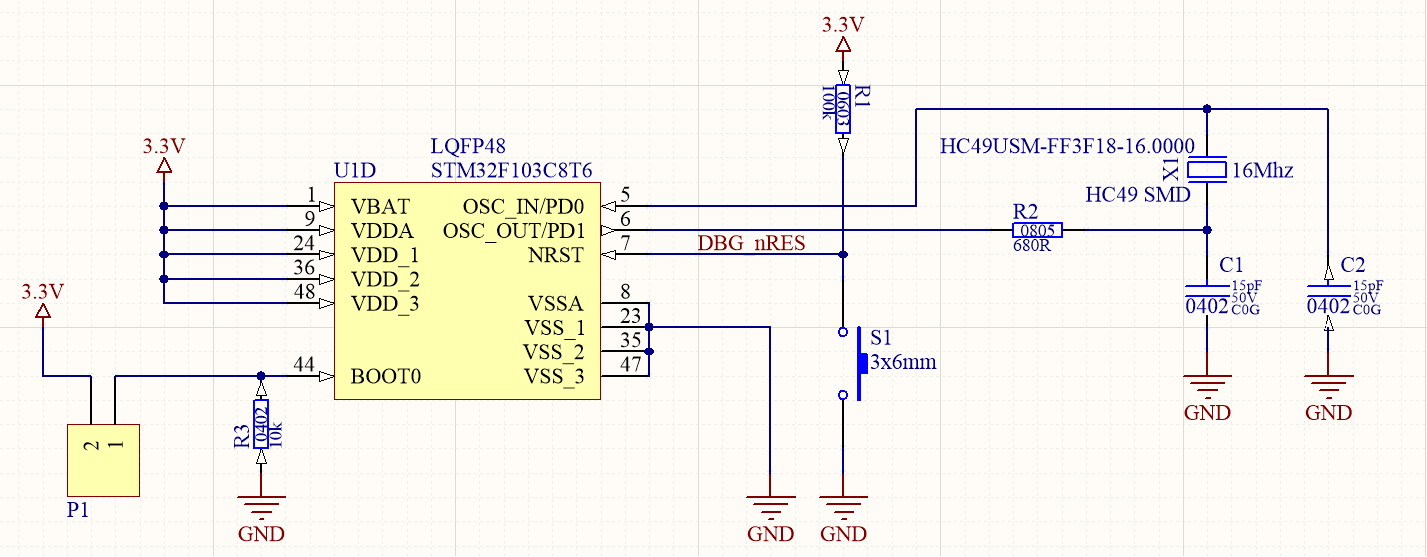
\includegraphics[width=0.65\paperwidth]{images/MCU_oscillator_and_reset.png}
    \centering
    \caption{Schemat połączenia wyprowadzeń mikrokontrolera STM32F103C8 odpowiedzialnych za resetowanie i układ rezonatora}
    \label{MCU_STM32_osc_and_reset}
\end{figure}


\chapter{Oprogramowanie }

Zadaniem opracowanego oprogramowania jest:
\begin{enumerate}
    \item sterowanie przełączaniem urządzeń docelowych i jego sygnalizacją
    \item implementacja komunikacji poprzez USB lub UART
    \item resetowanie urządzeń docelowych
\end{enumerate}

\section {Oprogramowanie układowe multipleksera SWD}
Kod został napisany w języku C.
Składa się z kilku modułów:
\begin{enumerate}
    \item sterownik USB - moduł ten został dostarczony w większości przez producenta. Odpowiada za komunikację zgodnie z protokołem USB-CDC. Dzięki niemu multiplekser zgłasza się do urządzenia nadrzędnego jako wirtualny port szeregowy. Dodatkowo zaimplementowano w nim bufor kołowy. Dzięki temu uzyskano prosty w obsłudze interfejs komunikacyjny o charakterze strumienia. Z racji pakietowej transmisji protokołu USB, dla wysyłania ciągu znaków w jednym pakiecie, wymagane było umieszczenie procesu w tle, który dopiero po otrzymaniu znacznika końca pakietu ładował dane do bufora kołowego. Dla prostoty i z racji małej ilości danych wysyłanych przez multiplekser SWD, każdy znak wysyłany w stronę komputera jest wysyłany w osobnym pakiecie.
    \item sterownik interfejsu UART - oparty częściowo na warstwie abstrakcji sprzętowej dostarczonej przez producenta. Dodano obsługę bufora kołowego. Obsługa interfejsu UART oparta jest na przerwaniach (przerwanie niepustego bufora wejściowego oraz przerwanie pustego bufora wyjściowego). Urządzenie wykorzystuje to samo API (Application Programming Interface) co wirtualny port szeregowy USB opisany wyżej.
    \item sterownik przełączników oraz wskaźników urządzeń - Ta część oprogramowania skupia się na ustawieniu wyjść za pomocą sterownika GPIO tak, aby linie sygnałowe z programatora zostały przekierowane na odpowiednie urządzenie. Dodatkowo wybrane urządzenie wskazywane jest poprzez diody umieszczone koło gniazd prowadzących do urządzeń docelowych.
    \item interfejs wiersza poleceń (Command Line Interface - CLI) - nasłuchuje znaków odebranych jednocześnie z USB jak i UART (połączone strumienie wejściowe) i po znalezieniu znaku nowej linii przeszukuje ciąg znaków pod kątem znaku odstępu. Znaki przed nim to nazwa komendy, a znaki do nowej linii to argument. Proces CLI działający w tle przeszukuje listę jednokierunkową komend i jeśli znajdzie tę komendę - wykonuje ją przekazując jej argument. Jeśli komenda nie została znaleziona - zwraca informację o błędzie na połączony strumień wyjścia, który rozdziela się na USB i UART.
    \item sterownik przycisków - korzysta ze sterownika GPIO i NVIC dostarczonych przez producenta. czeka na przerwanie pochodzące od przycisków i w zależności od linii przerwania wykonuje odpowiednią funkcję.
\end{enumerate}

\begin{center}
\begin{figure}[H]
\centering
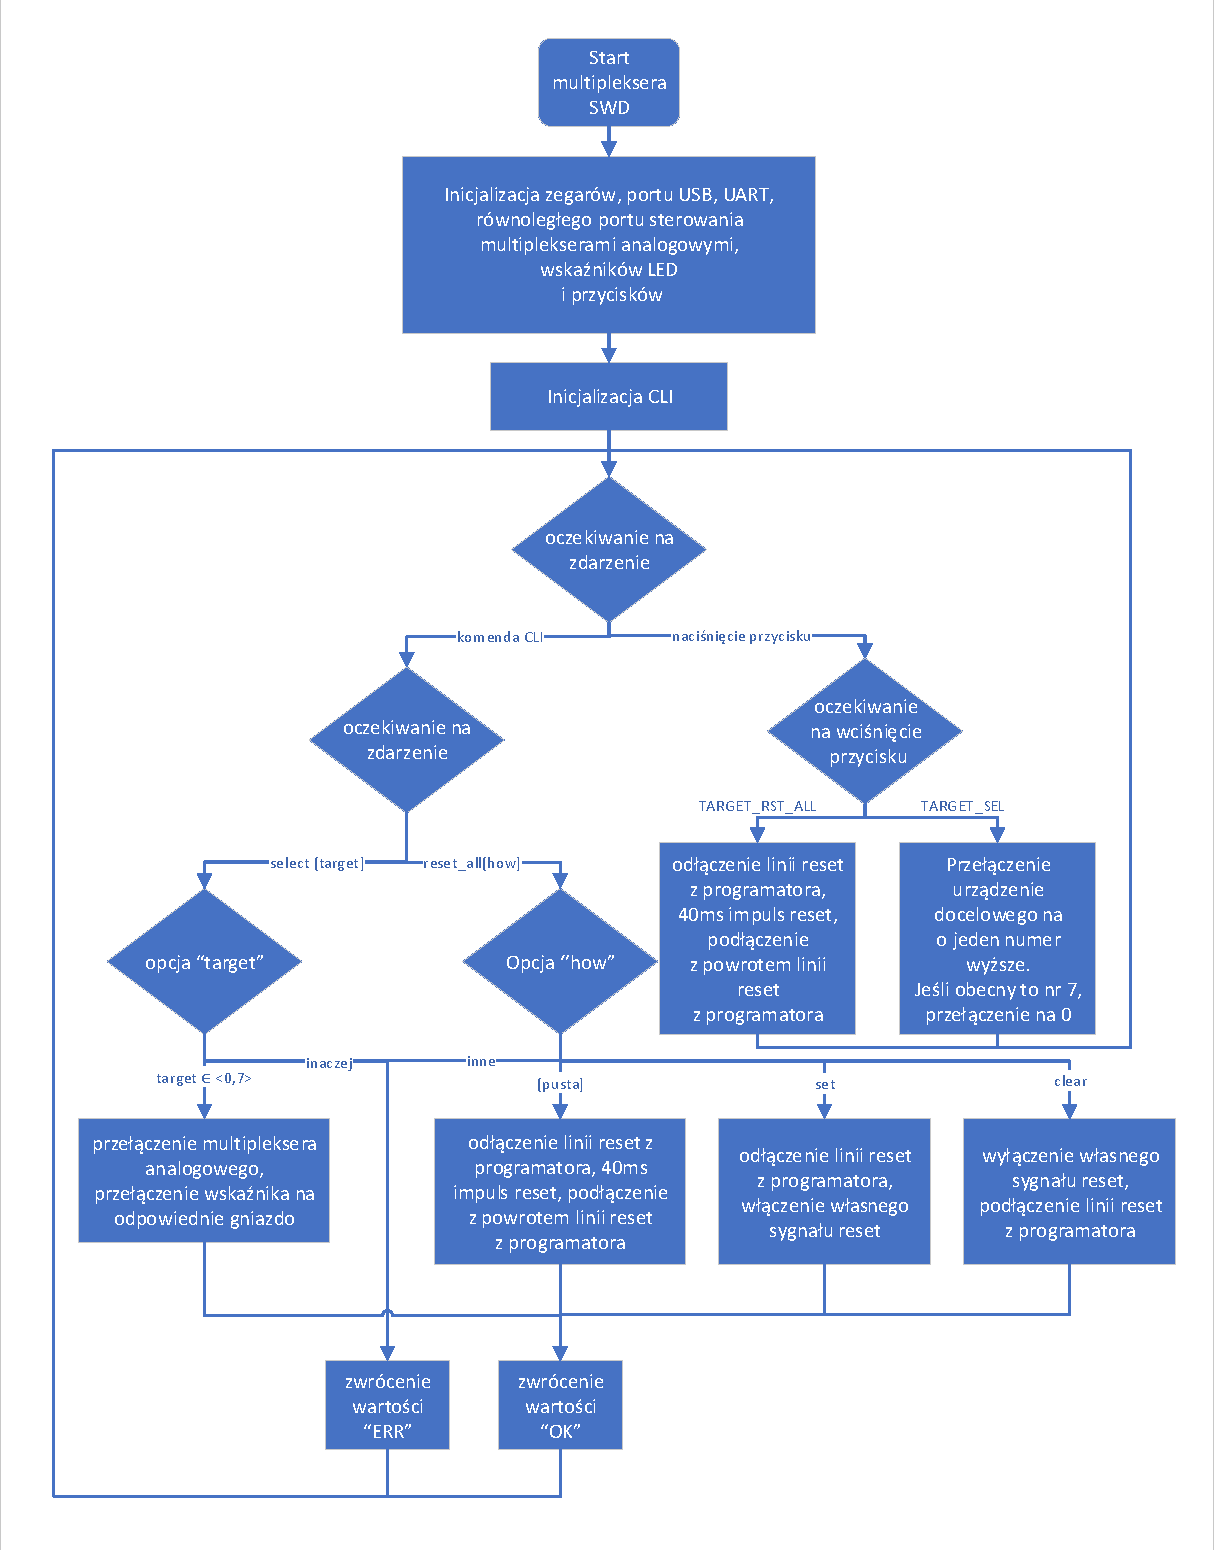
\includegraphics[width=0.72\paperwidth]{images/Mux_blokowy_soft.pdf}
\caption{Schemat blokowy oprogramowania układowego multipleksera SWD}
\label{SWD_MUX_software_block_diagram}
\end{figure}
\end{center}



\section {Oprogramowanie PC}
Multiplekser SWD jest urządzeniem, które wykorzystywane jest na etapie rozwoju i testów oprogramowania wbudowanego. Z racji dużej popularności interpretera Python w tej dziedzinie, najwygodniejsze jest użycie właśnie tego języka do wydawania prostych poleceń przez port szeregowy. Ponadto czyni to program łatwo przenośnym pomiędzy różnymi systemami operacyjnymi po drobnych modyfikacjach wynikających np. z różnicy komend używanych w różnych systemach operacyjnych.

Wymagania oprogramowania to:
\begin{enumerate}
    \item System operacyjny Microsoft Windows
    \item Interpreter Python 3
    \item oprogramowanie J-Link Commander (od wersji v6.60, dodatkowo wymagane dodanie folderu  \emph{bin} z katalogu instalacyjnego oprogramowania J-Linka do zmiennej środowiskowej PATH w systemie operacyjnym)
\end{enumerate}


Oprogramowanie na PC spełnia 3  główne funkcje:
\begin{enumerate}
    \item Zmiana urządzenia docelowego. Program sprawdza, czy bieżące urządzenie jest inne niż wybrane. Jeśli tak, wysyłana jest komenda do multipleksera SWD. Jeśli bieżące urządzenie jest w stanie resetu indywidualnego, jest on wyłączany.
    \item Resetowanie wszystkich urządzeń jednocześnie. Polega na wysłaniu komendy \emph{reset\_all} z opcją podaną w argumencie. Domyślnie nie ma opcji.
    \item Resetowanie bieżącego urządzenia. Realizowane przez skrypt uruchamiany w J-Link Commander. Funkcja przyjmuje argument analogicznie do funkcji \emph{reset\_all}
    \item Przesyłanie oprogramowania do urządzenia docelowego. Funkcja tworzy i uruchamia skrypt w J-Link Commander. Obsługiwany format pliku to ".hex".
\end{enumerate}

Biblioteka napisana jest w taki sposób, aby każdemu urządzeniu docelowemu można było zdefiniować inny plik zawierający jego oprogramowanie. Ponadto przewiduje możliwość programowania różnych modeli urządzeń. 




\chapter{Montaż urządzenia i testy końcowe}

\section{Montaż}
Montaż został przeprowadzony w większości metodą reflow z zastosowaniem pasty lutowniczej bezołowiowej. Pojedyncze elementy przewlekane lutowane były spoiwem z 40-60\% ołowiu. Z powodu braku odpowiednich części w miejsce kryształu kwarcowego w montażu powierzchniowym umieszczono odpowiednik w montażu przewlekanym bez wiercenia otworów.

\section{Testy}
Testy przeprowadzono podłączając do multipleksera urządzenia docelowe oparte na mikrokontrolerach Silicon Labs z rodziny EZR32 opartych na rdzeniach ARM Cortex-M4. 
Test został zautomatyzowany z pomocą języka programowania Python.
Scenariusz testu przedstawia się następująco:
\begin{enumerate}
    \item Wstępne sprawdzenie przełączania urządzeń docelowych i interfejsu komunikacyjnego.\\ 
    Polega na szybkim przełączeniu urządzeń docelowych od 0 do 7 i od 7 do 0. Nadzoru dokonuje osoba uruchamiająca test. Polega to na sprawdzeniu, czy po kolei zaświeciła się każda z diod. Jeśli którekolwiek z poleceń wysłanych do multipleksera SWD zakończy się opowiedzią inną niż OK z jego strony, następuje ponowne przesłanie komendy. Ponowne wysyłanie może się odbyć do 4 razy. Po tym program jest zatrzymywany z powodu nieobsłużonego wyjątku.
    \item Test resetowania.\\
    Sprawdzana jest reakcja multipeksera SWD jak i urządzeń docelowych. W tym wypadku urządzenie docelowe mrugało diodą podczas sekwencji startowej.
    \item Próba zaprogramowania urządzeń.\\
    Program próbuje zaprogramować dziesięciokrotnie każde z urządzeń. W przypadku wystąpienia błędu programowania, inkrementowany jest licznik błędów dla konkretnego urządzenia docelowego. Po zakończeniu wgrywania programu na każde z urządzeń docelowych sprawdzono, czy nastąpiła sekwencja testowa sygnalizująca poprawne ponowne uruchomienie. Pod koniec program testujący wypisuje podsumowanie testu w postaci ilości błędów podczas wgrywania oprogramowania. Jeśli nastąpi problem komunikacyjny na linii komputer - multiplekser SWD, program jest zatrzymywany z komunikatem o wyjątku.
\end{enumerate}

Cały test wykonany z użyciem komunikacji USB odbył się pomyślnie, bez jakichkolwiek błędów. Maksymalna możliwa do uzyskania szybkość sygnału zegarowego SWCLK to \SI{9}{MHz}.
Ponowne wykonanie testu poprzez wbudowany w J-Linka UART zakończyło się niepowodzeniem. Ciężko zdiagnozować przyczynę, jednak najprawdopodobniej jest to błąd powstały podczas montażu.

Wynikiem testów było zaobserwowanie poniższych problemów kwalifikujących się do poprawy w następnych wersjach płytki drukowanej:
\begin{enumerate}
    \item Niedziałająca opcjonalna komunikacja poprzez wbudowany w programator port UART. \\
    Obecna wersja płytki drukowanej zawiera konwertery poziomów logicznych TXS0102YZPR. Układ ten posiada obudowę DSBGA, która nie ma odsłoniętych wyprowadzeń, co utrudnia montaż oraz późniejszą diagnozę błędów w działaniu urządzenia. Płytka drukowana nie zawiera żadnych wyprowadzeń kontrolnych do których dałoby się w łatwy sposób podpiąć analizator stanów logicznych celem weryfikacji poprawności montażu. Z powodu braku potrzeby silnej eliminacji kosztów multipleksera SWD, można zastosować układ w innej obudowie (układy z serii TXS0102 są dostępne również w obudowach VSSOP).
    \item Brak wstępnej polaryzacji linii VtRef.\\
    Programator J-Link podciąga linię VtRef do masy. W przypadku niepodpiętego urządzenia docelowego do któregoś z gniazd i przełączeniu multipleksera SWD właśnie na ten port, niemożliwe będzie odebranie przez multiplekser SWD komendy, gdyz układ konwersji poziomów logicznych nie będzie działał prawidłowo. Rozwiązaniem tego problemu jest wstępna polaryzacja linii VtRef napięciem 1.8V poprzez rezystor \SI{1}{\Mohm}
    \item Celem uzyskania wyższej szybkości transmisji interfejsu SWD należy wymienić filtry przeciwprzepięciowe zabezpieczające gniazda urządzeń docelowych na odpowiedniki bez filtra dolnoprzepustowego, lub na takie z dużo wyższą częstotliwością odcięcia (co najmniej \SI{30}{MHz}).
    
\end{enumerate}

\chapter{Model 3D  urządzenia i fotografie stanowiska testowego}

\begin{figure}[H]
    \centering
    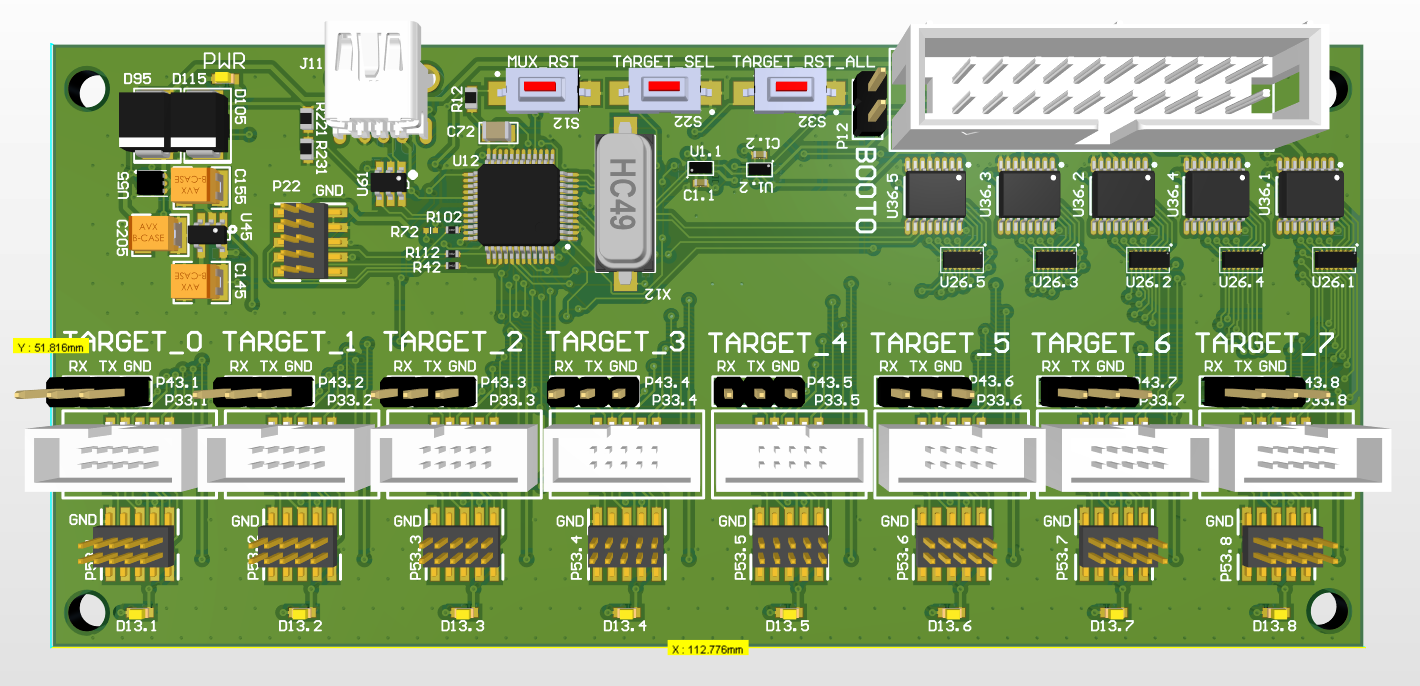
\includegraphics[width=0.75\paperwidth]{images/front_PCB.png}
    \caption{Model 3D płyty PCB widziany od przodu}
    \label{PCB_front}
\end{figure}

\begin{figure}[H]
    \centering
    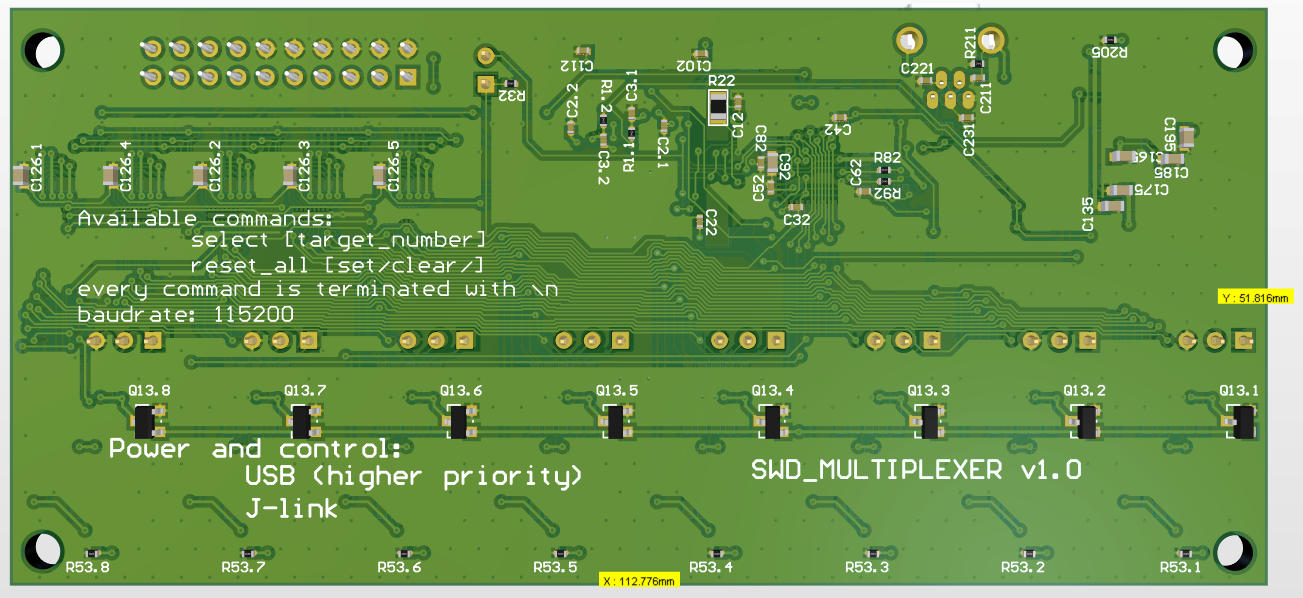
\includegraphics[width=0.75\paperwidth]{images/back_PCB.png}
    \caption{Model 3D płyty PCB widziany od tyłu}
    \label{PCB_back}
\end{figure}

\begin{figure}[H]
    \centering
    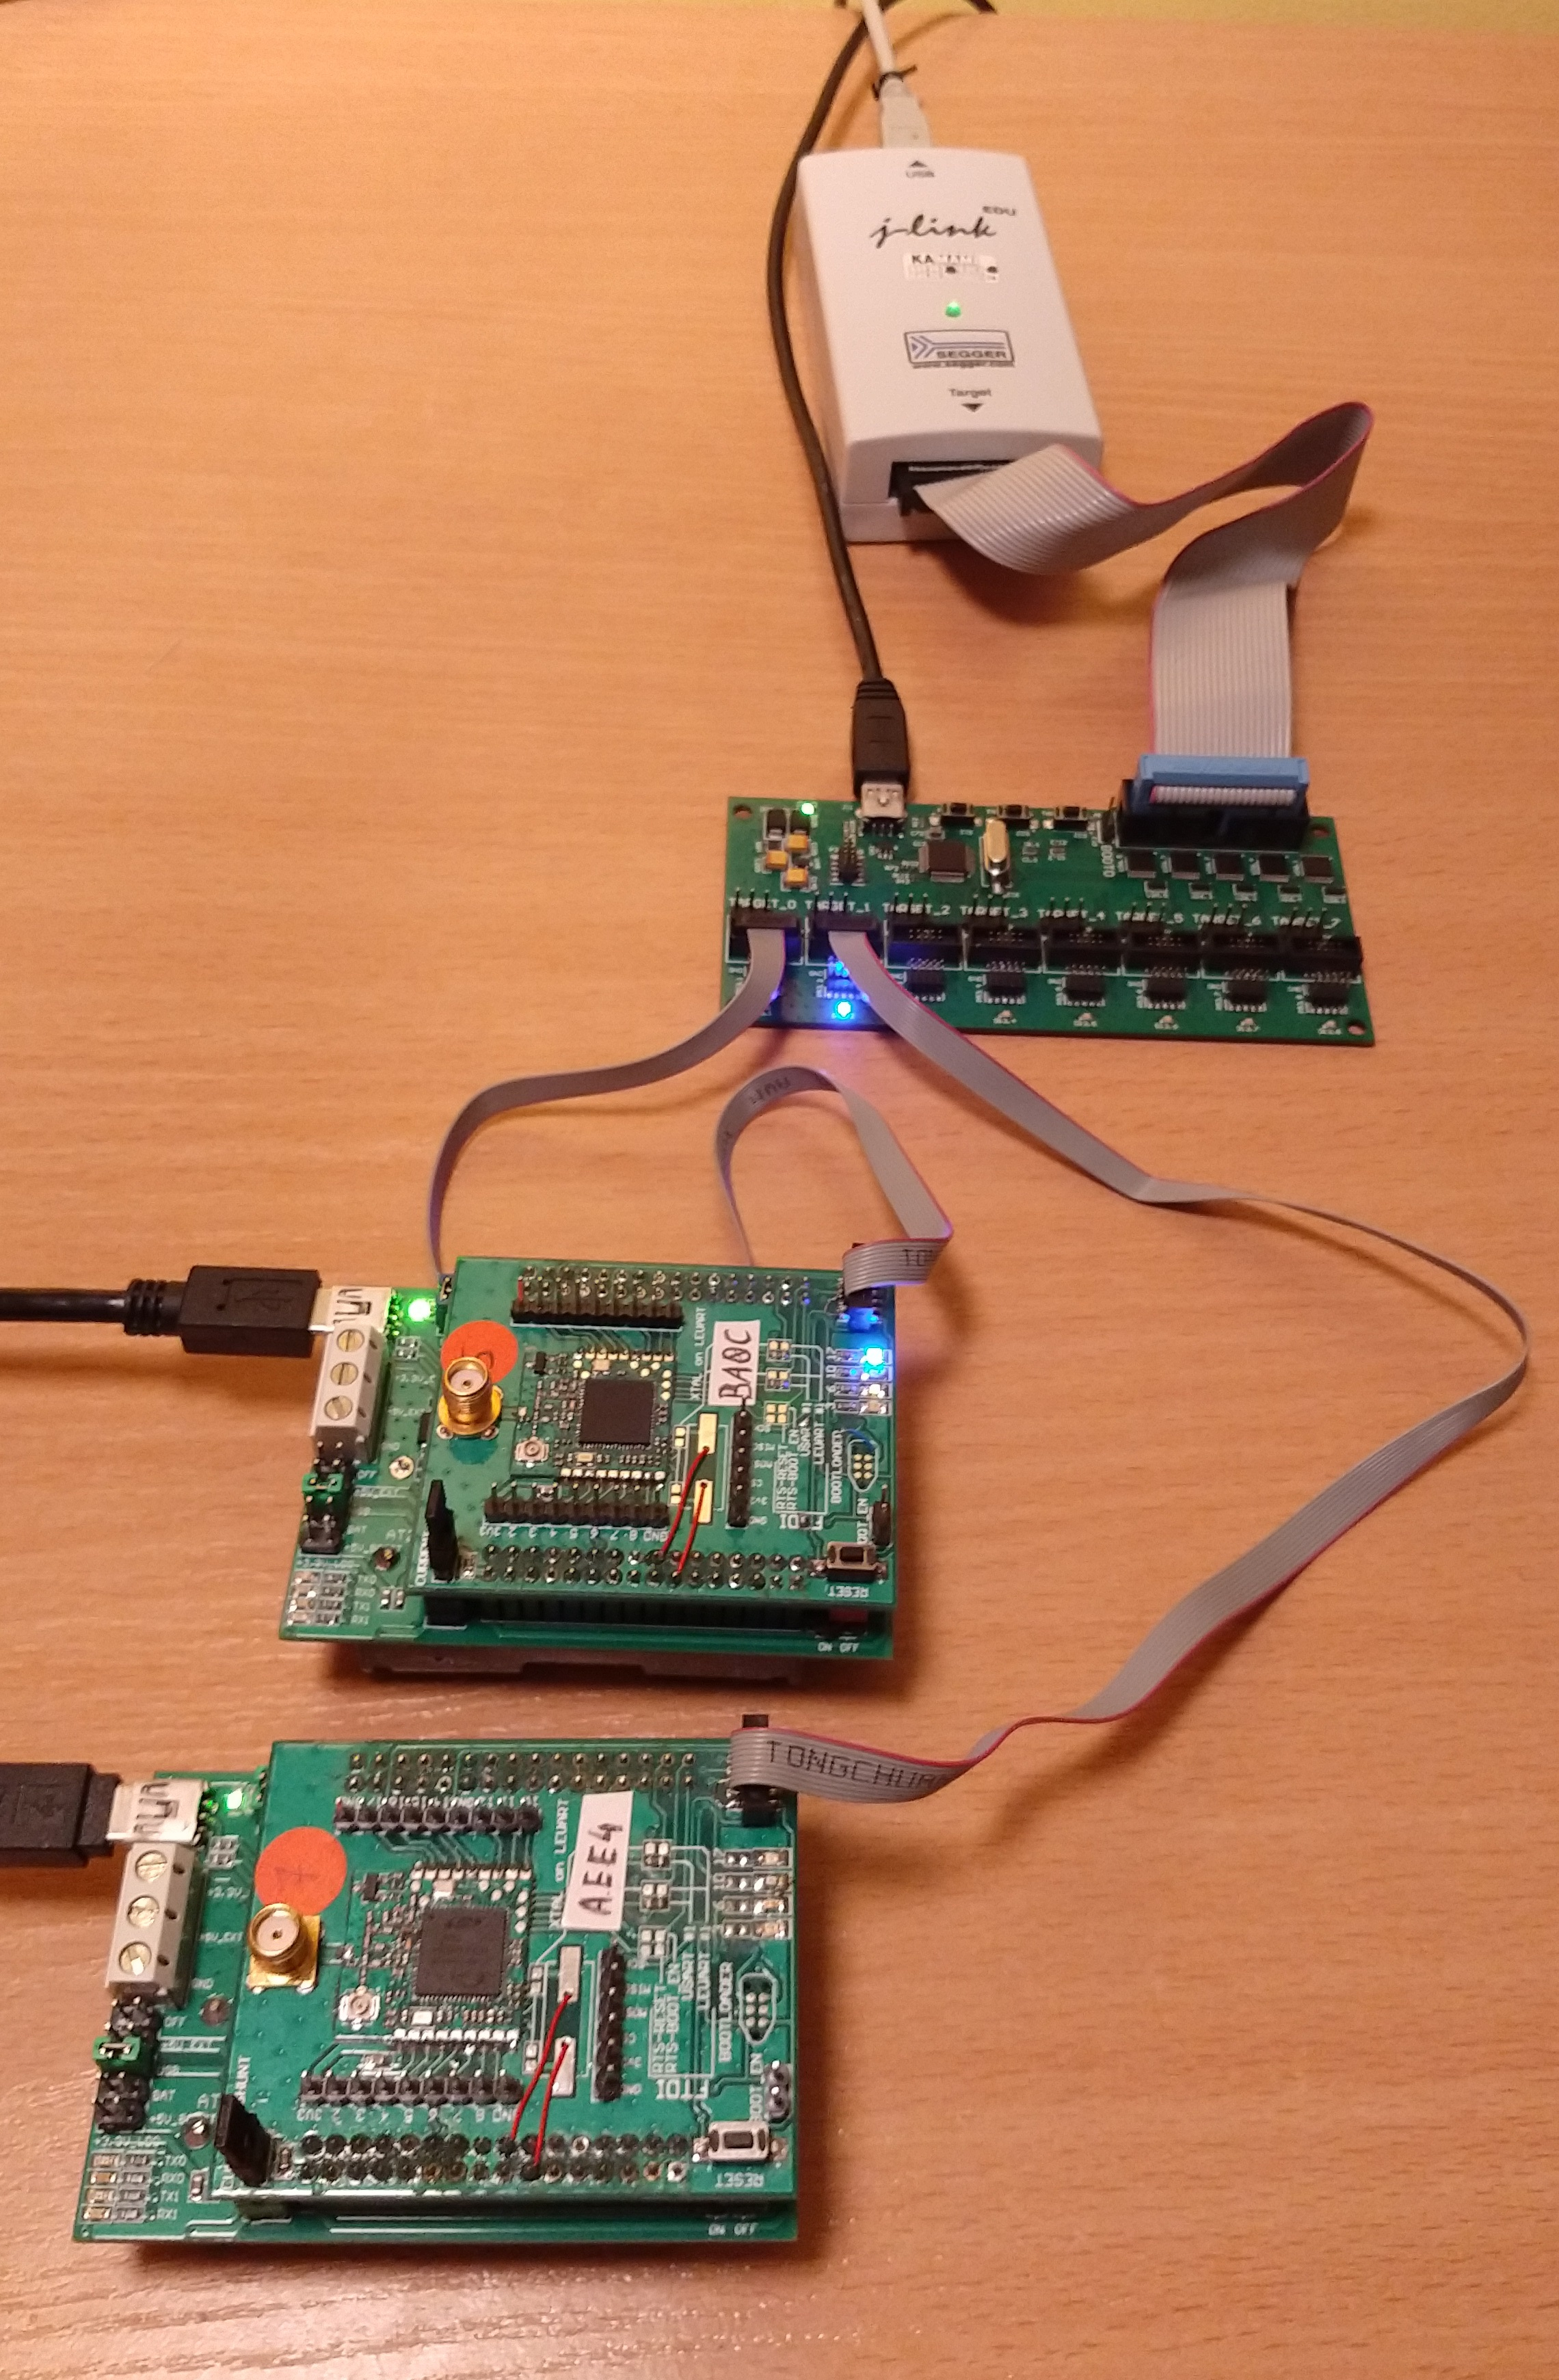
\includegraphics[width=0.75\paperwidth]{images/test_bench.jpg}
    \caption{Zdjęcie stanowiska testowego}
    \label{testbench_photo}
\end{figure}
\chapter{Podsumowanie}

W ramach pracy wykonano następujące czynności:
\begin{enumerate}
    \item Zaprojektowanie i wykonanie sprzętowe część projektu.\\
    Projekt wykonano w programie Altium Designer 19 przy użyciu biblioteki elementów elektronicznych przygotowanych w zespole Bezprzewodowych Sieci Kontrolno-Pomiarowych Katedry Elektroniki AGH. W czasie trwania projektu rozbudowano także wspomnianą bibliotekę o nowe podzespoły, których wcześniej nie zawierała. 
    \item Opracowanie oprogramowania układowego multipleksera SWD.\\ Oprogramowanie jest łatwo przenośne pomiędzy rodziną mikrokontrolerów STM32 zawierających interfejs USB, ponieważ użyto w nim bibliotek HAL producenta.
    \item Przygotowanie oprogramowania sterującego multiplekserem SWD z poziomu komputera z systemem operacyjnym Windows.\\
    Oprogramowanie to zawiera kontrolę błędów zarówno po stronie interfejsu użytkownika jak i multipleksera SWD. Pomaga to wykryć np błędy w połączeniu multipleksera SWD, urządzeń docelowych lub programatora. W prosty sposób można dodać funkcjonalność w postaci obsługi innych programatorów i wsparcie pozostałych systemów operacyjnych wspieranych przez środowisko Python 3.
    \item Testy działania urządzenia pod kontrolą komputera.\\
    Próbie został podjęty zarówno multiplekser SWD jak i program kontrolujący urządzenie z poziomu komputera klasy PC.
\end{enumerate}

Płytka PCB została wykonana w fabryce na podstawie projektu wyeksportowanego do plików formatu gerber, a jej wymiary to \SI{112.78}{mm} x \SI{51.8}{mm}.
Posiada otwory montażowe umożliwiające prosty montaż płyty w obudowie.

Zdecydowaną zaletą urządzenia jest uproszczenie i minimalizacja kosztów produkcji i testowania oprogramowania systemów wbudowanych zawierających interfejs SWD.

Praca opublikowana zostanie jako otwartoźródłowy projekt na platformie GitHub.




\appendix
\printbibliography
\chapter{Słowniczek pojęć}
Lista ważnych, używanych w pracy pojęć:
\begin{enumerate}
\item 
\textbf{GDB Serwer} -  program komputerowy, który pośredniczy pomiędzy programem GNU Debugger a systemem docelowym (urządzeniem docelowym) W przypadku tej pracy program zarządza programatorem komunikującym się z urządzeniem docelowym
\item 
\textbf{SWD} - Swrial Wire Debug - interfejs komunikacyjny pomiędzy programatorem i mikrokontrolerem z rdzeniem ARM Cortex-M
\item 
\textbf{interfejs} - wspólne połączenie, poprzez które dwa lub więcej oddzielnych elementów wymienia się informacjami w ściśle określony sposób.
\item 
\textbf{urządzenie docelowe} - w przypadku pracy urządzenie oparte na mikrokontrolerze z rdzeniem ARM Cortex-M.
\item 
\textbf{mikrokontroler} – układ cyfrowy z wyspecjalizowanym  mikroprocesorem i niezbędnymi do  jego samodzielnej pracy urządzeniami zawartymi w jednym układzie scalonym. Źródło:\cite{mikrokontroler_definicja}\\
\item
\textbf{USB} - Uniwersal Serial Bus - interfejs uniwersalnej magistrali szeregowej ustandaryzowany przez USB Implementers Forum
\item
\textbf{multiplekser} - Przełącznik zrealizowany w postaci układu elektronicznego. Najczęściej jest to układ scalony. Wyprowadzenie o adresie wybranym na złączach sterujących połączone jest z wyprowadzeniem bez adresu. W przypadku multipleksera analogowego nie rozróżnia się wejść ani wyjść, ponieważ połączenie jest dwukierunkowe.
\item 
\textbf{programator} - urządzenie obsługujące interfejsy wymagane do zaprogramowania pamięci. Najczęściej używa się ich do programowania mikrokontrolerów. Najczęściej programatory wspierają również interfejsy diagnostyczne służące do  programowania i nadzorowania pracy urządzeń w systemie.
\item
\textbf{daisy chain} - Połączenie szeregowe urządzeń w topologii pierścienia. Polega na połączeniu wyjścia jednego urządzenia do wejścia drugiego.
\item
\textbf{UART} - nadajnik i odbiornik asynchronicznej transmisji szeregowej.

    
\end{enumerate}

\chapter{Streszczenie pracy}
Praca polegała na opracowaniu i wykonaniu układu multipleksera SWD - urządzenia pozwalającego na sekwencyjne programowanie pamięci  do ośmiu mikrokontrolerów poprzez interfejs SWD przy użyciu tylko jednego programatora.\\
Urządzenia docelowe muszą posiadać wsparcie dla interfejsu SWD oraz wtyczkę w standardzie CoreSight10, lub WSN Connector.\\
Programator musi działać w standardzie ARM JTAG 20.
Praca multipleksera SWD jest być kontrolowana przez program oparty o język Python 3.\\ 
Program ten wysyła komendy  i odbiera potwierdzenia przez port szeregowy.\\
Używanie multipleksera SWD ma na celu:
\begin{enumerate}
    \item uproszczenie stanowiska testowego
    \item zmniejszenie kosztów stanowiska testowego
    \item dodanie funkcji jednoczesnego resetu urządzeń docelowych
    \item zautomatyzowanie procesu wgrywania oprogramowania do pamięci urządzeń docelowych
    \item eliminację wpływu czynnika ludzkiego podczas używania platformy testowej
\end{enumerate}

Wykonanie projektu zakończyło się sukcesem w przeważającej części. Nie działa jedynie dodatkowa komunikacja z multiplekserem SWD poprzez wbudowany w J-Linka (programator) UART.

\end{document}
